\documentclass[tikz,border=2pt]{standalone}
\usepackage{amsmath}
\usepackage{pgfplots}
\pgfplotsset{compat=1.18}

\begin{document}
% A bounded sequence need not converge, but inside the strip |a_n| <= M some subsequence (red)
% must settle down: here the even-indexed terms converge to 1.
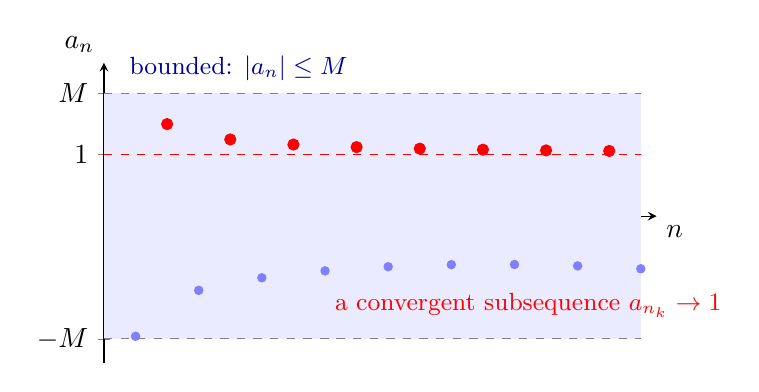
\begin{tikzpicture}
	\begin{axis}[
		axis lines=middle,
		xmin=0, xmax=17.5,
		ymin=-2.4, ymax=2.5,
		xtick={1,5,10,15}, ytick={-2,1,2}, yticklabels={$-M$,$1$,$M$},
		xlabel={$n$}, ylabel={$a_n$},
		xlabel style={below right}, ylabel style={above left},
		clip=false,
		width=8.6cm, height=5.4cm
		]
		\fill[blue!8] (axis cs:0,-2) rectangle (axis cs:17,2);
		\addplot[gray, dashed, domain=0:17] {2};
		\addplot[gray, dashed, domain=0:17] {-2};
		\addplot[red, dashed, domain=0:17] {1};
		\addplot[only marks, mark=*, mark size=1.5pt, blue!50, samples at={1,3,5,...,17}] {(-1)^x*(1+1/x)+0.3*sin(deg(3*x))};
		\addplot[only marks, mark=*, mark size=2pt, red, samples at={2,4,6,...,16}] {(-1)^x*(1+1/x)};
		\node[blue!60!black, anchor=south west, font=\small] at (axis cs:0.5,2.05) {bounded: $|a_n|\le M$};
		\node[red, anchor=north west, font=\small] at (axis cs:7,-1.1) {a convergent subsequence $a_{n_k}\to 1$};
	\end{axis}
\end{tikzpicture}
\end{document}
